\section{Generative Models}

\subsection{Generative Models}

Generative models 隶属于 unsupervised learning 的范畴，其数据集没有标签。其目的是根据输入学会一种数据集的分布，并生成具有这种分布的新的图像。

\begin{figure}[H]
    \centering
    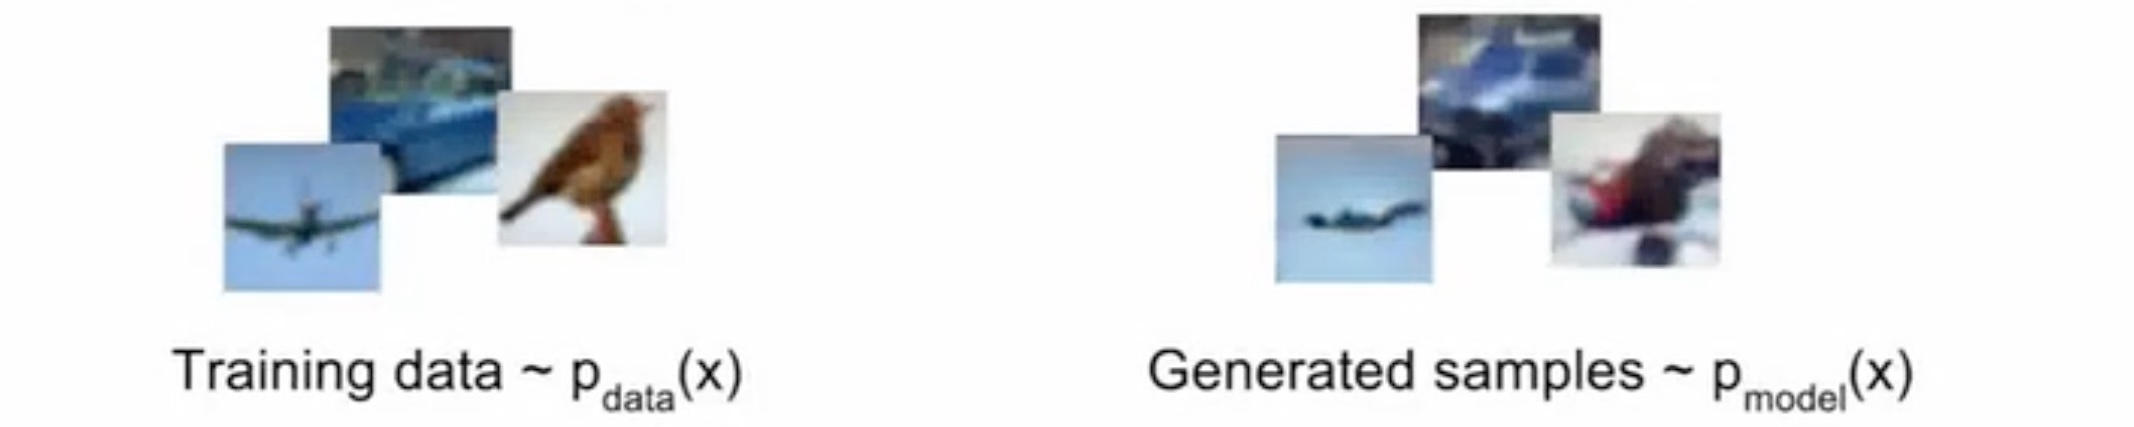
\includegraphics[width=0.8\linewidth]{figs/chapter8/generative.jpg}
\end{figure}

\subsection{Pixel RNN \& Pixel CNN}

Pixel RNN 和 Pixel CNN 都属于 \textbf{Fully visible belief network}，其思想是对于图像 $x$，计算其似然 $p_\theta(x)$：
\[
p_\theta(x)=\prod_{i=1}^n p_\theta(x_i\mid x_1,\ldots,x_{i-1})
\]
其中 $x_i$ 是 $x$ 的一个像素。$p_\theta(x_i\mid x_1,\ldots,x_{i-1})$ 含义是，在已经生成像素点 $x_1\ldots x_{i-1}$ 的条件下，下一个像素点为 $x_i$ 的概率。那么根据极大似然法的思想，我们想生成一个好的图像 $x$，目标就是最大化似然函数 $p_\theta(x)$.

这跟网络有什么关系呢？上式的计算未免过于复杂，而我们知道神经网络善于对一个复杂的计算过程建模，因此我们可以设计一些网络达到目的。

\paragraph{Pixel RNN}

我们从左上角开始，按照下图所示顺序生成新的像素：

\begin{figure}[H]
    \centering
    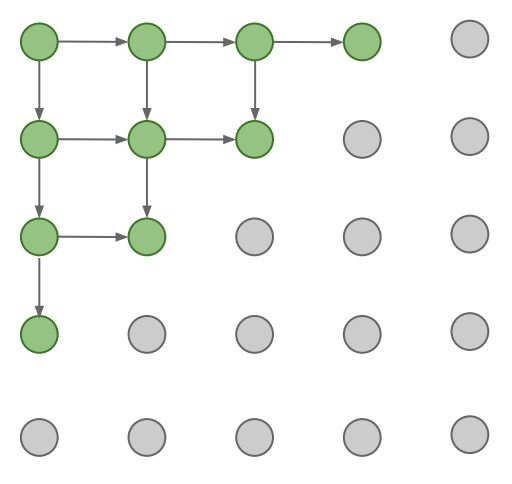
\includegraphics[width=0.2\linewidth]{figs/chapter8/pixelrnn.jpg}
\end{figure}

自然而然地，这个时序过程可以用 RNN/LSTM 来完成。

其缺点是每个像素是顺次生成的，这导致网络的生成速度较慢，其训练速度也慢。

\paragraph{Pixel CNN}

把 RNN 换成 CNN，根据周围像素生成新的像素。

\begin{figure}[H]
    \centering
    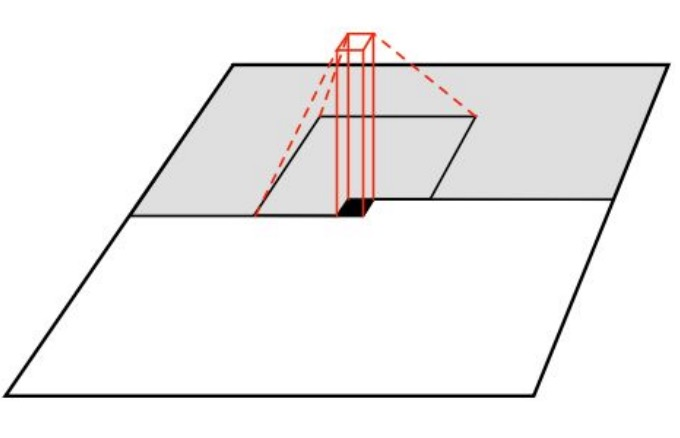
\includegraphics[width=0.2\linewidth]{figs/chapter8/pixelcnn.jpg}
\end{figure}

训练比 Pixel RNN 快，但生成依旧是顺次生成，速度依旧较慢。

\subsection{Variational  Autoencoders (VAE)}

\paragraph{Autoencoders}

在学习 VAE 之前，我们首先需要了解 Autoencoders.

Autoencoders 是一种 unsupervised 的 dimensionality reduction 的方法。其思想是，用一个 CNN 将输入数据 $x$ 降维为 $z$，然后再用一个 CNN 将降维后的数据 $z$ 恢复为原大小 $\hat x$，并定义 loss function 为：$||x-\hat x||^2$，这样在训练后，前一个 CNN 就可以作为数据降维的 encoder 了。注意这个过程并没有使用标签，所以这是 unsupervised 的。

Autoencoders 可以用于 supervised model 的初始化，帮助模型的学习。

\begin{figure}[H]
    \centering
    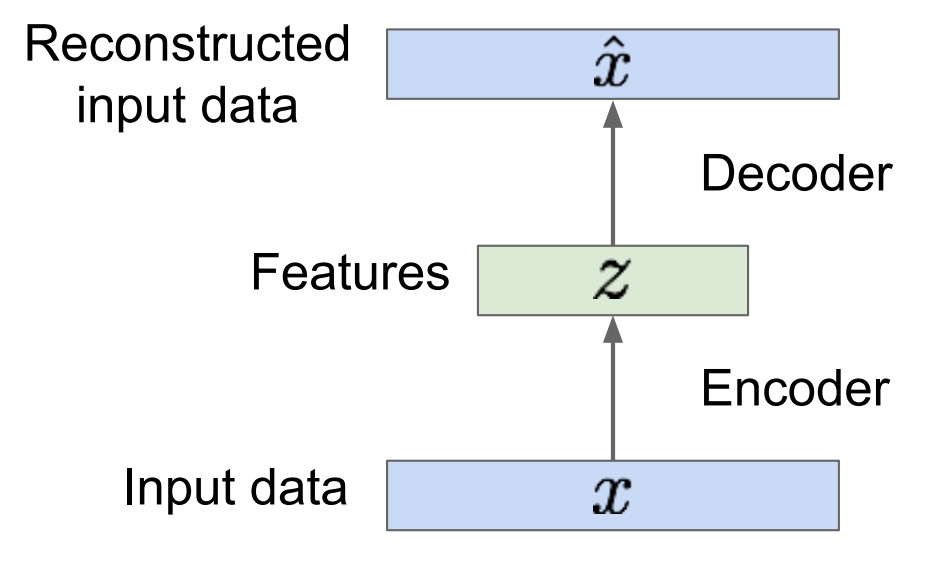
\includegraphics[width=0.35\linewidth]{figs/chapter8/autoencoders.jpg}
\end{figure}

\paragraph{VAE}

我们假设真实数据 $\{x^{(i)}\}_{i=1}^N$ 是由一个未知的、隐藏的 $z$ 采样得到的，也就是说，给定 $z^{(i)}$，$x^{(i)}$ 采样自概率分布 $p_\theta(x\mid z^{(i)})$，而这里的 $z^{(i)}$ 又采样自一个先验概率分布：$p_\theta(z)$.
\begin{figure}[H]
    \centering
    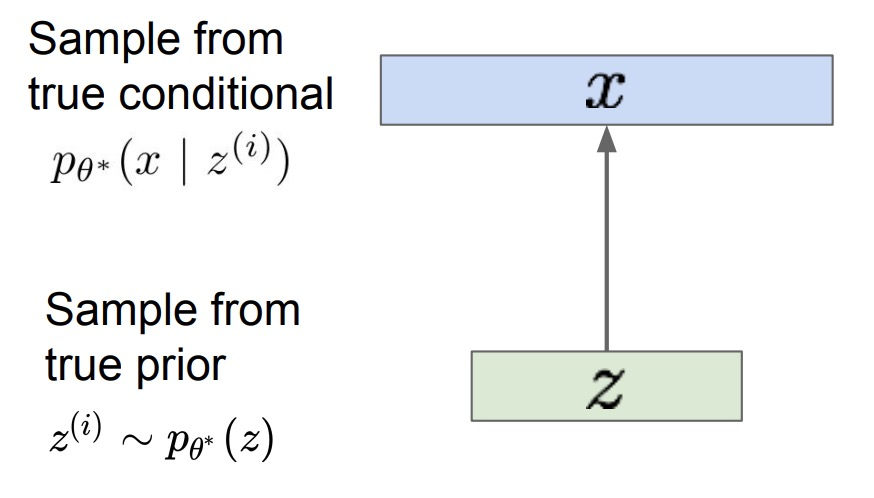
\includegraphics[width=0.35\linewidth]{figs/chapter8/vae.jpg}
\end{figure}

我们可以合理地选取高斯分布为 $z$ 的先验分布；又由于 $p_\theta(x\mid z^{(i)})$ 是一个复杂的东西，所以我们可以用一个 decoder network 对它进行建模。那如何训练这个神经网络呢？不同于 Fully visible belief network，VAE 将似然写作：
\[
p_\theta(x)=\int p_\theta(z)p_\theta(x\mid z)\mathrm dz
\]

根据极大似然法的思想，最大化这个似然函数就是训练神经网络的过程了。

这时问题出现了，因为积分的存在，我们无法处理 $p_\theta(x)$ 这个函数，也就无法训练神经网络；我们也没法处理后验分布：$p_\theta(z\mid x)=p_\theta(x\mid z)p_\theta(z)/p_\theta(x)$。

对于第二个问题，我们再定义一个神经网络 $q_\phi(z\mid x)$ 去近似 $p_\theta(z\mid x)$：

\begin{figure}[H]
    \centering
    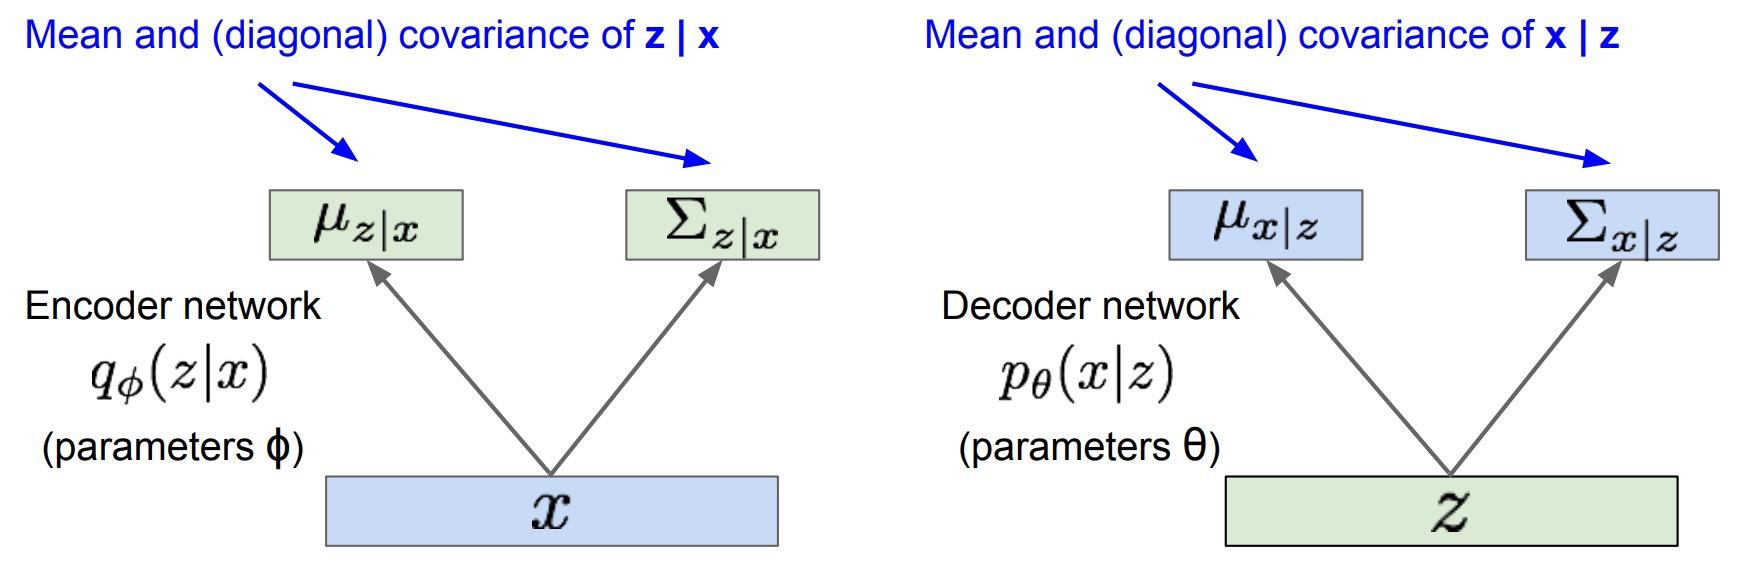
\includegraphics[width=0.7\linewidth]{figs/chapter8/vae2.jpg}
\end{figure}

两个神经网络的输出都是均值和方差，如此，在 inference 阶段，我们可以选取以该均值和方差为统计量的正态分布作为采样的概率分布。

对第一个问题的解决方法是，我们训练一个 $p_\theta(x)$ 的下界：
\begin{align*}
\log p_\theta(x^{(i)})&=\mathbb E_{z\sim q_\phi(z\mid x^{(i)})}\left[\log p_\theta(x^{(i)})\right]\\
&=\mathbb E_z\left[\log\frac{p_\theta({x^{(i)}\mid z})p_\theta(z)}{p_\theta(z\mid x^{(i)})}\right]\\
&=\mathbb E_z\left[\log\frac{p_\theta({x^{(i)}\mid z})p_\theta(z)}{p_\theta(z\mid x^{(i)})}\frac{q_\phi(z\mid x^{(i)})}{q_\phi(z\mid x^{(i)})}\right]\\
&=\mathbb E_z\left[\log p_\theta(x^{(i)}\mid z)\right]-\mathbb E_z\left[\log\frac{q_\phi(z\mid x^{(i)})}{p_\theta(z)}\right]+\mathbb E_z\left[\log\frac{q_\phi(z\mid x^{(i)})}{p_\theta(z\mid x^{(i)})}\right]\\
&=\mathbb E_z\left[\log p_\theta(x^{(i)}\mid z)\right]-D_{KL}(q_\phi(z\mid x^{(i)})||p_\theta(z))+D_{KL}(q_\phi(z\mid x^{(i)})||p_\theta(z\mid x^{(i)}))\\
&\geqslant \mathbb E_z\left[\log p_\theta(x^{(i)}\mid z)\right]-D_{KL}(q_\phi(z\mid x^{(i)})||p_\theta(z))
\end{align*}
于是乎，我们训练神经网络的过程，就是最大化这个下界 $\mathcal L(x^{(i)},\theta,\phi)=\mathbb E_z\left[\log p_\theta(x^{(i)}\mid z)\right]-D_{KL}(q_\phi(z\mid x^{(i)})||p_\theta(z))$ 的过程。如何理解这个过程呢？最大化 $\mathcal L(x^{(i)},\theta,\phi)$，就要最大化第一项——即努力重新构造出输入数据，以及最小化第二项——即努力使得近似后验分布接近于我们预定的先验分布。综上，我们的训练过程如下：

\begin{figure}[H]
    \centering
    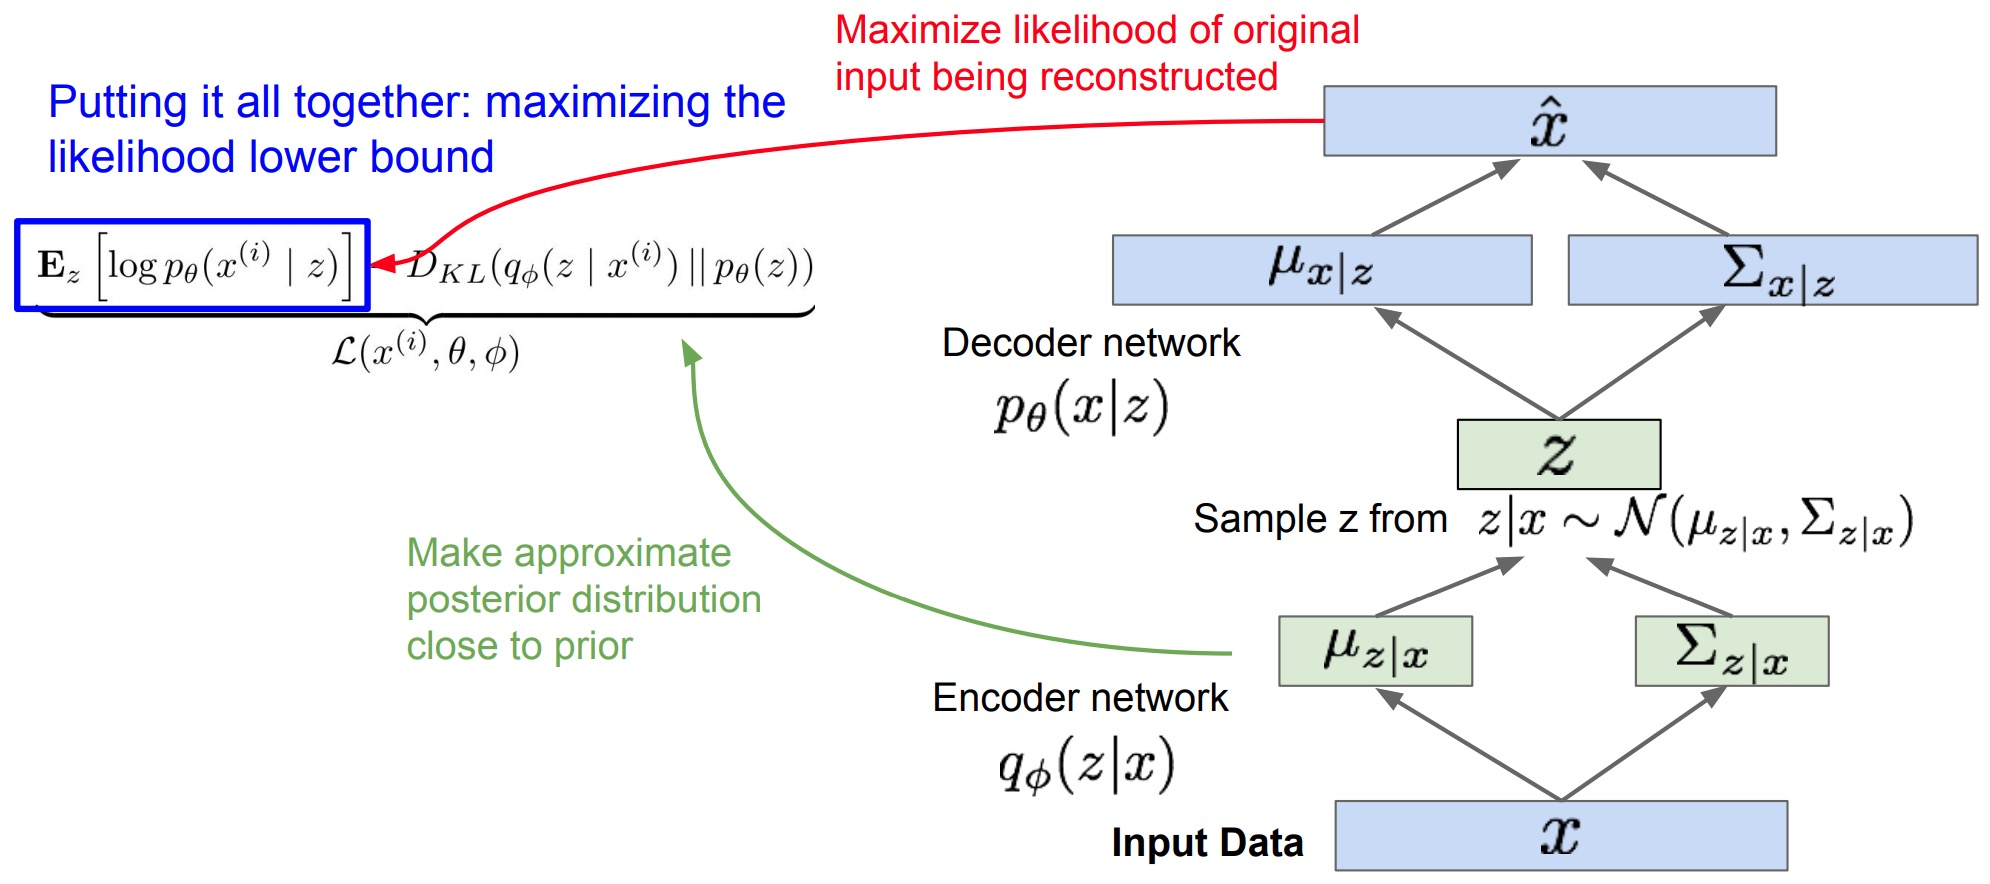
\includegraphics[width=0.8\linewidth]{figs/chapter8/vae3.jpg}
\end{figure}

现在我们训练好了一个 VAE 网络，就可以用它来生成数据了。从 $z\sim N(0,I)$ 对 $z$ 进行采样，然后用训练的 decoder network 得到 $\mu_{x\mid z}$ 和 $\Sigma_{x\mid z}$，随后从 $x\mid z\sim N(\mu_{x\mid z},\Sigma_{x\mid z})$ 得到生成的数据 $\hat x$：

\begin{figure}[H]
    \centering
    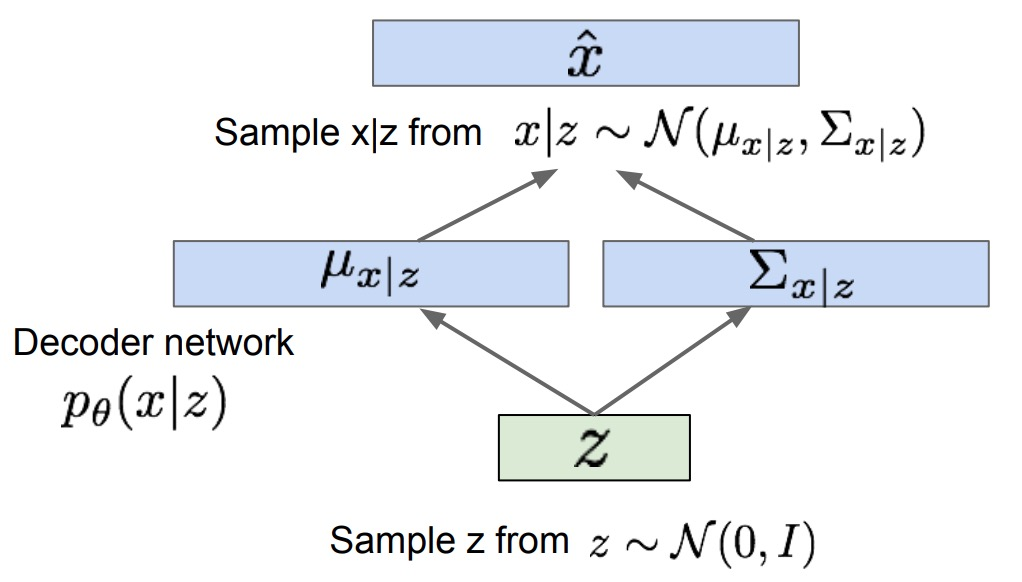
\includegraphics[width=0.4\linewidth]{figs/chapter8/vae4.jpg}
\end{figure}

以下是生成 MNIST 数字的 VAE，选取 $z$ 为 $2$ 维时可以得到：

\begin{figure}[H]
    \centering
    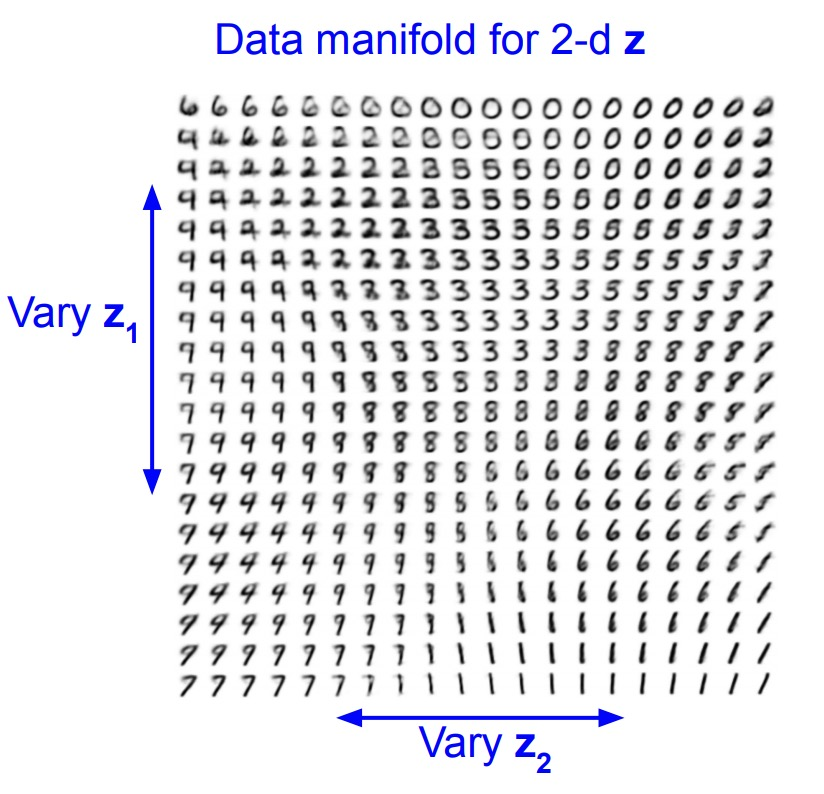
\includegraphics[width=0.4\linewidth]{figs/chapter8/vae5.jpg}
\end{figure}


\subsection{GANs}

PixelCNNs 和 VAEs 都显式地对概率密度函数 $p_\theta(x)$ 进行了定义，我们是否可以不给出一个显式的概率密度函数呢？GANs 网络就是这样的。

我们没有直接的方法从训练集里找出一个概率分布并据此采样以生成新的图像，但我们能从一个简单分布采样，例如随机噪声；随后我们不断改变这个简单的分布，以最终逼近真正的分布。这个复杂的过程显然用神经网络建模是最好不过的了：

\begin{figure}[H]
    \centering
    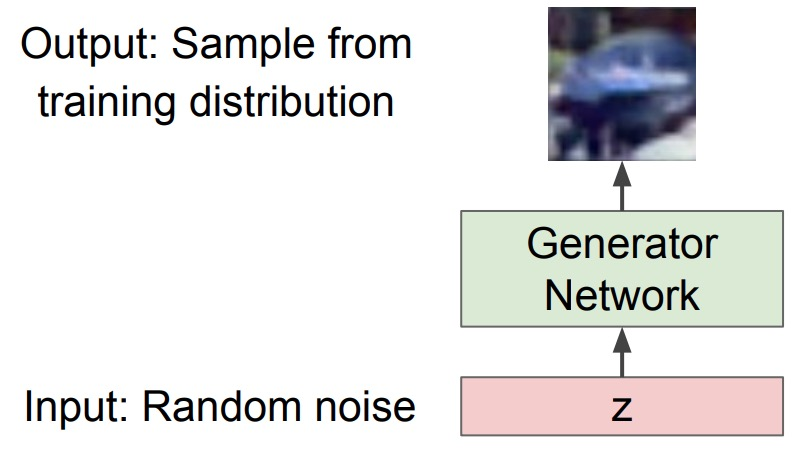
\includegraphics[width=0.4\linewidth]{figs/chapter8/gan.jpg}
\end{figure}

那么我们如何训练这个神经网络呢？方法是用两个神经网络进行博弈——Generator 负责生成新的图像，Discriminator 负责辨别输入图像是真的还是假的（输出真的概率）。训练时 Generator 的目标是尽可能地骗过 Discriminator，而 Discriminator 的目标就是不被 Generator 骗到。

\begin{figure}[H]
    \centering
    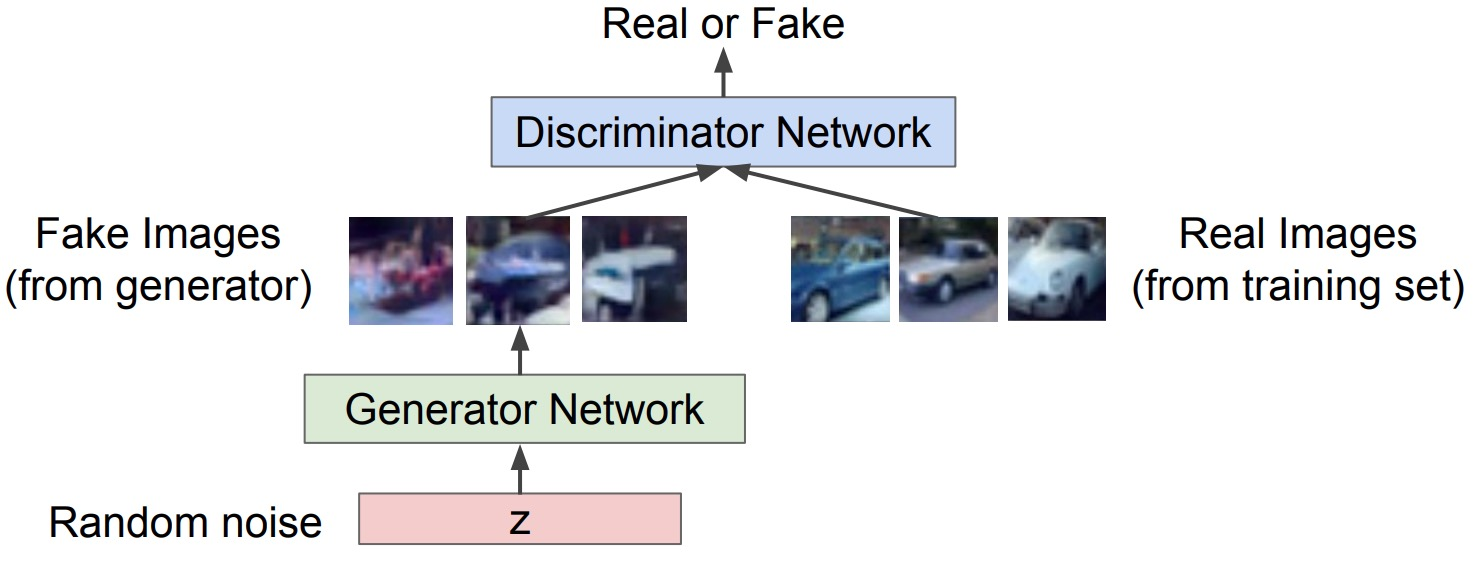
\includegraphics[width=0.6\linewidth]{figs/chapter8/gan2.jpg}
\end{figure}

我们的目标函数定义为 Minimax objective function：
\[
\min_{\theta_g}\max_{\theta_d}\left[\mathbb E_{x\sim p_{data}}\ln D_{\theta_d}(x)+\mathbb E_{z\sim p(z)}\ln(1-D_{\theta_d}(G_{\theta_g}(z))) \right]
\]
先看内层 $\max$ 的部分，第一项中，$x$ 取自真实分布，$D_{\theta_d}(x)$ 是 Discriminator 认为真的概率，所以这一项是要最大化真实图像是真的的概率；第二项中，$z$ 取自生成网络，$1-D_{\theta_d}(G_{\theta_g}(z))$ 是 Discriminator 认为假的概率，所以这一项是要最大化假图像是假的的概率。因此，内层值越高，代表 Discriminator 越准确，这正好不是 Generator 希望看到的，所以外层套一个 $\min$，表示 Generator 希望 Discriminator 的最大得分尽可能低。这正是所谓的 minimax 算法。

训练时这个目标函数可以拆成两部分，对 Discirminator，用梯度上升使得：
\[
\max_{\theta_d}\left[\mathbb E_{x\sim p_{data}}\ln D_{\theta_d}(x)+\mathbb E_{z\sim p(z)}\ln(1-D_{\theta_d}(G_{\theta_g}(z)))\right]
\]
对 Generator，用梯度下降使得：
\[
\min_{\theta_g}\mathbb E_{z\sim p(z)}\ln(1-D_{\theta_d}(G_{\theta_g}(z)))
\]
因为前一项与 $\theta_g$ 无关，所以只有这后一项。

然而在实践中，优化这个目标函数并不能工作得很好。这是因为 $y=\ln(1-x)$ 的特性是在 $x$ 接近 $0$ 时梯度较小，$x$ 接近 $1$ 时梯度很大，于是在 Generator 这里，生成的图像很假的时候学习较慢，生成的图像已经很逼真的时候学习反而很快，不符合我们的预期。因此，我们改用梯度上升训练 Generator，使得：
\[
\max_{\theta_g}\mathbb E_{z\sim p(z)}\ln(D_{\theta_d}(G_{\theta_g}(z)))
\]
这样梯度就符合我们的预期了。

总结一下，训练 GANs 的流程为：

\begin{figure}[H]
    \centering
    \tcbox[colframe=black, colback=white, boxrule=0.5pt, sharp corners]{
        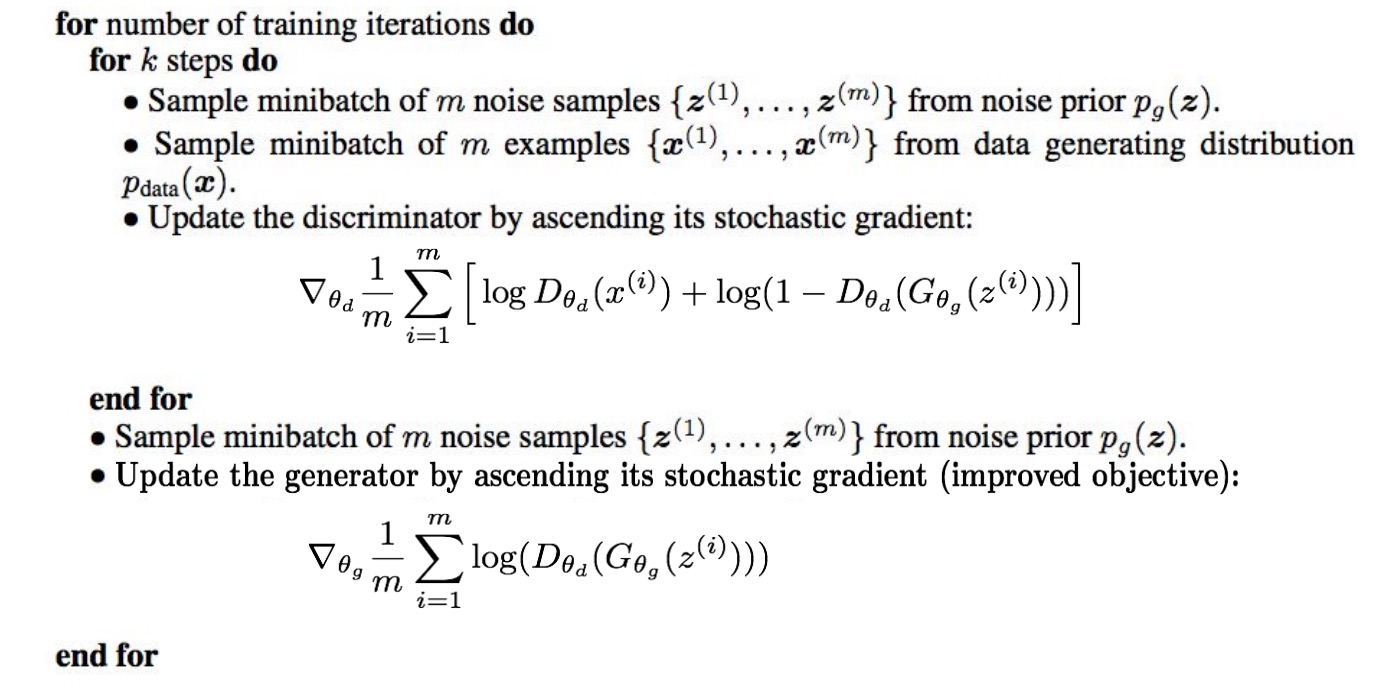
\includegraphics[width=0.9\linewidth]{figs/chapter8/gantrain.jpg}
    }
\end{figure}
